\subsection{Relationship between cell size and growth rate.}

While our analysis suggest that ribosomes set the maximum growth rate,  our
estimates also point to a more important role for ribosomes in setting  cell
size and in the maintenance of steady-state growth  when considered in light of
a number of recent studies.  We use the remainder of the text to consider these,
beginning with cell size. The relationship between cell size and growth rate has
long been of interest in the study of bacteria, particularly following the now
decade-old observation that cell volume appears to increase exponentially with
growth rate; known as Schaechter's growth law  \citep{schaechter1958,
taheriaraghi2015}. Wild-type \textit{E. coli} growing at relatively fast growth
rates, show a remarkably constant cell cycle time ($t_{cyc}$, referring to the C
+ D periods of DNA replication and cell division), as shown in
\FIG{translation_ecoli_partA}(A) for the data reproduced from \citep{si2017}.
With a constant cell cycle time, the exponential scaling in size has long been
considered a direct consequence of cells initiating replication at a constant
volume per origin. However, the particular mechanism that governs this
relationship, and even the question of whether the change in average cell size
is truly exponential  have remained under debate \citep{si2017, harris2018}.

Under the simplest of strategies, for example, given the constraint set by
Equation 3 it would seem most appropriate for the cell to only adjust its
proteome through the synthesis of additional ribosomes. In contrast, it is clear
that a large portion of the proteome increases in absolute abundance. Cells
maintain a linear scaling between size and number of origins that is robust to a
remarkable array of perturbations \citep{si2017}. In
\FIG{translation_ecoli_partA}(B) we show this linear trend for ribosomes  from
each of the  proteomic data sets.  $\langle$\# ori$\rangle$ is determined by how
often replication forks must be initiated per cell cycle to maintain
steady-state growth, and is calculated from 2$^{\tau_{cyc} / \tau}$, where
$\tau_{cyc}$. Here we have estimated $\langle$\# ori$\rangle$ from the
measurements of \cite{si2017} for wild-type cells grown under nutrient
limitation.

Through our estimates in the sections on the central dogma, it is
apparent that the processes of transcription (i.e. synthesis of mRNA) and
translation are unlikely limiting steps in the process of doubling the
cell mass. This argues that as DNA replication beings to parallelize, the
proteome should only change in ways that reflect the change in DNA gene dosage
and mRNA distribution, and any additional aspects of gene regulation.
The total amount of protein synthesized over a cell cycle is nevertheless
determined by $R \times r_t / \lambda$. Since protein accounts for most of
the cellular dry mass \citep{bremer2008, basan2015}, cell size will also vary
in proportional to this. The relationship between cell size and growth rate,
however, will then depend only on how the cell varies its ribosomal
fraction, as highlighted by Equation 3.

\subsubsection{Exponential relationship between cell size and growth rate is
set by ribosomal abundance at moderate to fast growth rates.}

It is notable that the majority of ribosomal proteins and rRNA operons are found
closer to the DNA origin. For a relatively constant cell cycle time $t_{cyc}$
and in particular, for a constant DNA replication period $t_C$, parallelized DNA
replication has the important consequence that it will skew absolute gene dosage
and mRNA abundance in favor of genes closer to the origin \citep{scholz2019}
[more cites] (\FIG{translation_ecoli_partA}(C)). This raises the possibility
that for moderately fast growth rates (above about 0.5 h$^{-1}$), where these
time scales are nearly constant, that the increased number of chromosomal
origins can be viewed as a way for the cell to skew its ribosomal abundance.
Importantly, alternative solutions such as simply increasing the expression of
ribosomes for a particular $\langle$\# ori$\rangle$ will not be possible if rRNA
synthesis is nearly limiting. Biasing DNA dosage in this manner  also provides a
means to maintain levels of expression for most other proteins that are
nonetheless needed for growth, as we've seen throughout our estimates.

We were unaware, however, of whether such the skew in gene dosage at fast growth
materializes at the proteomic level. In \FIG{translation_ecoli_partA}(D) we show
a running boxcar average (500 kbp window) of protein copy number as a function
of each gene's transcriptional start site (\FIG{translation_ecoli_partA}(D)).
While the protein copy numbers of individual proteins can vary substantially
across the entire chromosome, we nonetheless observe a bias in expression under
fast growth conditions (dark blue lines). The dramatic change in protein copy
number near the origin is primarily due to the increase in ribosomal protein
expression. This trend is in contrast to slower growth conditions (yellow) where
the average copy number is much more uniform across the length of the chromosome.

\begin{figure*}
    \begin{fullwidth}
    \centering{
        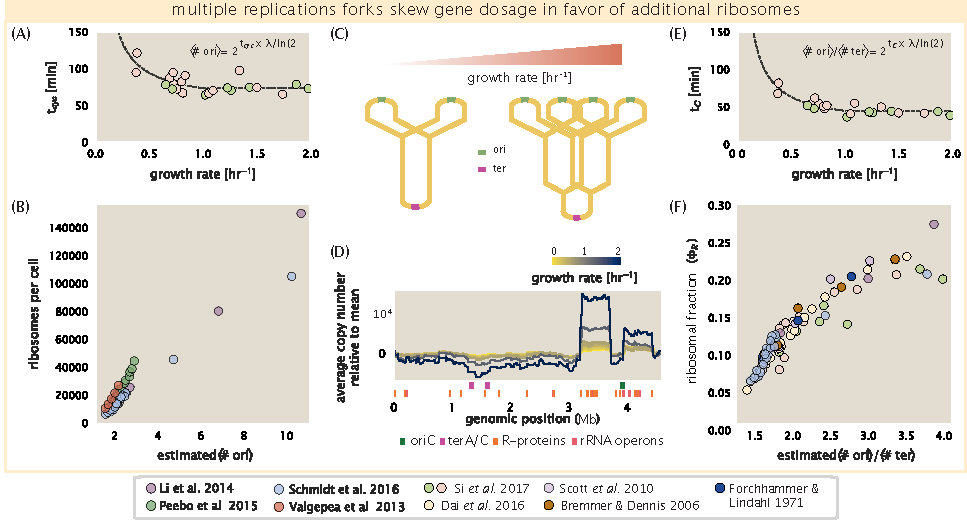
\includegraphics{main_figs/fig8_ribosome_growth_limit_ecoli_a.pdf}
        \caption{\textbf{Multiple replication forks skew gene dosage and
        ribosomal content.} (A) Experimental data from Si
        \textit{et al.} (2017). Dashed line shows fit to the data, which were
        used to estimate
        $\langle$\# ori$\rangle$. $t_cyc$ was assumed to vary in proportion to $tau$
        for doubling times great than 40 minutes, and then reach a minimum value of
        [fill in] minutes below this (see Supplemental Appendix X for additional details).
        Red data points
        correspond to measurements in strain MG1655, while light green points
        are for strain NCM3722.
        (B) Plot of the ribosome
        copy number estimated from the proteomic data against the estimated
        $\langle$\# ori$\rangle$ [NB: change to total protein abundance?].
        (C) Schematic shows the expected increase in
        replication forks (or number of ori regions) as \textit{E. coli} cells
        grow faster. (D) A running boxcar average of protein copy number is
        calculated for each each growth condition considered by Schmidt
        \textit{et al.}. A 0.5 Mb averaging window was used. Protein copy
        numbers are reported relative to their condition-specific means in order
        to center all data sets.
        (E)
        Experimental data from Si
        \textit{et al.} (2017) showing $t_C$ as a function of growth rate.
        Dashed line shows a best fit to the data, similar to part (A).
        (F) Plot compares our estimate of $\langle$\#
        ori$\rangle$ / $\langle$\# ter$\rangle$  to the experimental
        measurements of ribosomal abundance. Ribosomal fraction was approximated
        from the RNA/protein ratios of Dai \textit{et al.} (2016) (yellow) and
        Si \textit{et al.} (2017) (light red and light green) by the conversion
        RNA/protein ratio $\approx \Phi_R \cdot 2.1$. } \label{fig:translation_ecoli_partA}
    }
    \end{fullwidth}
\end{figure*}

%%%%%%%%%%%%%%%%%%%%%%%%
%%%%%%%%%%%%%%%%%%%%%%%%

%  It is only
% if ribosomal synthesis is rate limiting that the cell would need to vary
% [** As long as the cell maintains it's ability to synthesis ribosomes, i.e. not
% rate limiting, the cell will vary its ribosomal content according to number of origins
% it then follows  that cell size should scale with growth rate]
% ** However this breaks down when size  is not directly proportional to R.
% ***** It is only because R scales with number of origins that we get size vs. growth rate scaling.
% ***** (MAYBE) IF ribosomes are being synthesized in this regime essentially at their maximum amount,
% than it provides a possible explanation for the increase in ribosome abundance
%
%
% , albeit with a bias torward the origin of replication as discussed
% above. Indeed, most proteins exhibit a strong correlation with $\langle$\#
% ori$\rangle$, with the exception largely restricted to proteins involved in
% metabolism [make figure]. The total protein mass will then scale with
% $\langle$\# ori$\rangle$, which itself will be proportional to $R \times r_t
% \times \lambda$).
%
% Since size is largely determined by its protein and RNA mass, which account for
% over [70?] percent of total dry mass \citep{basan2015}, we can expect it to be
% proportional to the amount of protein synthesized over a cell cycle.  The
% specific scaling between $R$, and $\langle$\# ori$\rangle$, will depend on any
% growth dependent changes in both $r_t$ and any additional aspects of gene
% regulation. Nevertheless for an exponential increase in both $R$, and total
% protein content, there will be a linear increase in the ribosomal fraction
% $Phi_R$.  It then follows from Equation 2, that an increase in ribosomal
% fraction and proportionate increase in growth rate will be associated with an
% exponential increase in protein content and cell size.
%
% When ribosome synthesis is not rate limiting however, below about 0.5 hr$^{-1}$,
% ribosomal synthesis is no longer expected to be rate limiting and we
% have no reason to expect an exponential growth in size ?.
%
% %%%%%%%%%%%%%%%%%%%%%%%%%%%%
% %%%%%%%%%%%%%%%%%%%%%%%%%%%%

This result provides important evidence that although total protein content
scales with $\langle$\# ori$\rangle$, parallel DNA replication also skews the
proteome in favor of genes closer to the origin and in particular supports the
synthesis of additional ribosomes.   We can then view an increase in ribosomal
fraction $\Phi_R$ (and therefore, $\lambda$) as requiring a geometric increase
in total protein abundance that is proportional to $\langle$\# ori$\rangle$. For
\textit{E. coli}, which initiates chromosomal replication at fixed volume per
origin [cite], it then follows that the growth rate $\lambda$ will only increase
with an exponential increase in total protein.

\subsubsection{An exponential increase in chromosomal content provides shows
a diminishing benefit on growth.}

The ratio $\langle$\# ori$\rangle$ / $\langle$\# ter$\rangle$ can also be used
to consider this skew in chromosomal content. Quantitatively, this will depend
on how quickly the chromosome is replicated (i.e. its C period) relative the
cell's doubling time $\tau$ and this is given by 2$^{\tau_C / \tau}$. In
\FIG{translation_ecoli_partA}(C) we plot the measured $\tau_C$ versus $\tau$
(computed as $\tau = \log (2) / \lambda$), similarly using measurements on
wild-type \textit{E. coli} from  \citep{si2017}. In
\FIG{translation_ecoli_partA}(D) we plot the $\langle$\# ori$\rangle$ /
$\langle$\# ter$\rangle$ ratio against ribosomal fraction across a number of
recent measurements. Here we see that the ribosomal fraction doesn't increase as
much at higher $\langle$\# ori$\rangle$ / $\langle$\# ter$\rangle$. This may be
in part because not all rRNA operons are located exactly at the origin. However,
it also serves to highlight a diminishing  benefit on growth rate with
additional rounds of chromosomal initiation, which likely reflects  difficulty
in increasing the absolute number of ribosomes at fast growth.

% That work also measured the total RNA to protein ratio which
% reflects ribosomal abundance and we show that data along with other recent
% measurements from \cite{dai2016,dai2018}.
% Indeed, we find that the ribosomal
% fraction increases with $\langle$\# ori$\rangle$ / $\langle$\# ter$\rangle$
% (\FIG{translation_ecoli_partA}(C)). We note a systematic difference in the
% relative abundances from \cite{peebo2015} and \cite{valgepea2013} that was
% inconsistent with a number of other measurements of total RNA-to-protein ratios
% ($\approx \Phi_R$ x 2.1 \cite{dai2016}) and only show the data from
% \cite{schmidt2016} and \cite{li2014} for relative ribosome abundances (see
% supplemental section XX for a more complete discussion).

% Parallelized DNA replication represents a solution that allows  \textit{E. coli}
% to synthesize enough rRNA as it grows faster. That the cell appears to
% be synthesizing rRNA near its maximal rate at growth rates above about 0.5 h$^{-1}$
% may also have consequences on robust scaling  between
% cell size and $\langle$\# ori$\rangle$. As one example, when cells are exposed
% to sublethal doses of ribosome-inhibiting drugs like chloramphenicol, there is a
% notable increase in the cell's ribosomal fraction (grey points,
% \FIG{translation_ecoli_partA}(D)), but otherwise the cell is able to maintain
% its cell size according to $\langle$\# ori$\rangle$ \citep{si2017}. While the
% presence of chloramphenicol will inhibit protein synthesis, it will also allow
% for relatively higher rRNA synthesis due to the longer doubling time. If the
% cell can scale it ribosomal protein abundance through feedback from rRNA
% synthesis, than we would expect the relative abundance of ribosomes to increase
% according to the increase in rRNA synthesis. This type of feedback was
% considered long ago \citep{nomura1984} and we consider this possibility further
% in Supplemental Appendix XX.


% Below growth rates of about 0.5 h$^{-1}$ it becomes less clear whether  two regimes where this scaling relationship is likely to falter: (1)
% slow growth, below about 0.5 hr$^{-1}$ where the number of ribosomes $R$ no
% longer reflects the number of actively translating ribosomes, and (2) ????
% fastest growth due to limits on rRNA production)

% \subsection{Maximizing growth rate requires coordination of biosynthesis at all growth rates.}
%
% However, the mechanism behind growth rate control has remained elusive
% and has only been described at a phenomenological level.
%
% Here we attempt to place our observations across the proteomic data sets in the
% context of \textit{E. coli} maximizing its steady-state growth rate across a wide
% array of conditions.

% \section{Parellel DNA replication biases protein production in support of ribosome synthesis.}
%
% \textit{E. coli} cells grow by a so-called "adder" mechanism, whereby cells add
% a constant volume with each cell division \citep{taheriaraghi2015}. In
% conjunction with this, additional rounds of DNA replication are triggered when
% cells reach a critical volume per origin of replication
% (\FIG{translation_ecoli_partA}(A)). This leads to the classically-described
% exponential increase in cell size with growth rate \cite{schaechter1958, si2017,
% si2019}. In the context of maximizing growth rate, it is notable that the
% majority of ribosomal proteins and rRNA operons are found closer to the DNA
% origin.

% Given that cells must
% increase their total gene dosage of rRNA operons at faster growth rates, and the
% intimate relationship between ribosomal content and growth rate considered
% above, this raises the possibility that the increase in chromosomal content
% might simply be a means for the cell to tune biosynthesis according to its
% physiological state and the nutrient availability in its environment.

% While an increase in transcription has been observed for genes closer to the
% origin in rapidly growing \textit{E. coli} \citep{scholz2019}, we were unaware
% of such characterization at the proteomic level. In order to see whether there
% is a relative increase in protein expression for genes closer to the origin at
% faster growth, we calculated a running boxcar average (500 kbp window) of
% protein copy number as a function of each gene's transcriptional start site
% (\FIG{translation_ecoli_partA}(B)). While absolute protein copy numbers can vary
% substantially across the chromosome, we indeed observe a bias in expression
% under fast growth conditions (dark blue). The dramatic change in protein copy
% number near the origin is primarily due to the increase in ribosomal protein
% expression. This trend is in contrast to slower growth conditions (yellow) where
% the average copy number is more uniform across the length of the chromosome.
%
% \begin{figure*}
%     \begin{fullwidth}
%     \centering{
%         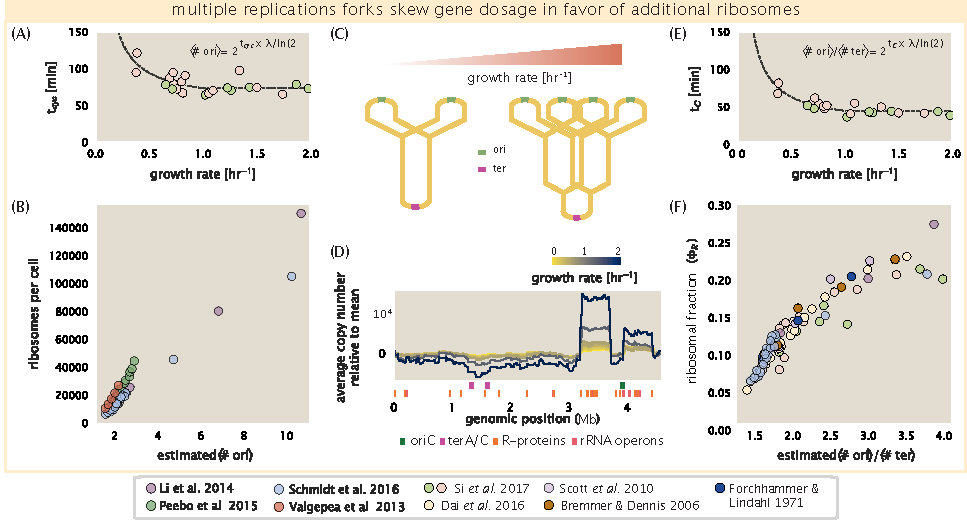
\includegraphics{main_figs/fig8_ribosome_growth_limit_ecoli_a.pdf}
%         \caption{\textbf{Multiple replication forks skew gene dosage and
%         ribosomal content.} (A) Schematic shows the expected increase in
%         replication forks (or number of ori regions) as \textit{E. coli} cells
%         grow faster. (B) A running boxcar average of protein copy number is
%         calculated for each each growth condition considered by Schmidt
%         \textit{et al.}. A 0.5 Mb averaging window was used. Protein copy
%         numbers are reported relative to their condition-specific means in order
%         to center all data sets. (C) and (E) show experimental data from Si
%         \textit{et al.} (2017) Solid lines show fits to the data, which were
%         used to estimate $\langle$\# ori$\rangle$ / $\langle$\# ter$\rangle$ and
%         $\langle$\# ori$\rangle$ [NB: to note fit equations]. Red data points
%         correspond to measurements in strain MG1655, while light green points
%         are for strain NCM3722. (D) Plot compares our estimate of $\langle$\#
%         ori$\rangle$ / $\langle$\# ter$\rangle$  to the experimental
%         measurements of ribosomal abundance. Ribosomal fraction was approximated
%         from the RNA/protein ratios of Dai \textit{et al.} (2016) (yellow) and
%         Si \textit{et al.} (2017) (light red and light green) by the conversion
%         RNA/protein ratio $\approx \Phi_R \cdot 2.1$. (F) Plot of the ribosome
%         copy number estimated from the proteomic data against the estimated
%         $\langle$\# ori$\rangle$.} \label{fig:translation_ecoli_partA}
%     }
%     \end{fullwidth}
% \end{figure*}

% \subsection{Ribosome abundance increases in proportion to expected rRNA gene dosage.}
%
% If ribosomal genes (rRNA and ribosomal proteins) are growth rate limiting and
% synthesized according to the available rRNA gene
% dosage and condition-dependent transcription rate, we expect that ribosomal
% abundance will vary in proportion to the increase in rRNA gene dosage. This will be related to $\langle$\# ori$\rangle$ and the $\langle$\# ori$\rangle$ /
% $\langle$\# ter$\rangle$ ratio.

% To estimate rRNA gene dosage, we considered the experimental data
% from \cite{si2017}, which inferred these parameters for cells under
% nutrient-limited growth. The ratio $\langle$\# ori$\rangle$ / $\langle$\#
% ter$\rangle$ depends on how quickly chromosomes are replicated relative the
% cell's doubling time $\tau$ and is given by 2$^{\tau_C / \tau}$. Here $\tau_C$
% is the time taken to replicate \textit{E. coli}'s chromosome, referred to as the
% C period of cell division.  In \FIG{translation_ecoli_partA}(C) we plot the
% measured $\tau_C$ versus $\tau$ (computed as $\tau = \log (2) / \lambda$), with
% data points in red corresponding to \textit{E. coli} strain MG1655, and blue to
% strain NCM3722. \cite{si2017} also measured the total RNA to protein ratio which
% reflects ribosomal abundance and we show that data along with other recent
% measurements from \cite{dai2016,dai2018}. Indeed, we find that the ribosomal
% fraction increases with $\langle$\# ori$\rangle$ / $\langle$\# ter$\rangle$
% (\FIG{translation_ecoli_partA}(C)). We note a systematic difference in the
% relative abundances from \cite{peebo2015} and \cite{valgepea2013} that was
% inconsistent with a number of other measurements of total RNA-to-protein ratios
% ($\approx \Phi_R$ x 2.1 \cite{dai2016}) and only show the data from
% \cite{schmidt2016} and \cite{li2014} for relative ribosome abundances (see
% supplemental section XX for a more complete discussion). For the data shown, the
% ribosomal fraction doesn't increase as much at higher $\langle$\# ori$\rangle$ /
% $\langle$\# ter$\rangle$. Since several rRNA operons are actually located
% approximately half-way between the origin and terminus, the trend may in part be
% a consequence of a diminishing increase in rRNA gene dosage at higher
% $\langle$\# ori$\rangle$ / $\langle$\# ter$\rangle$ ratios.


% protein fraction should
% increase in proportion to the average ratio of DNA origins to DNA termini
% ($\langle$\# ori$\rangle$ / $\langle$\# ter$\rangle$ ratio).

% we can make two related hypotheses about how their ribosome abundance should
% vary with chromosomal content. First, the ribosomal protein fraction should
% increase in proportion to the average ratio of DNA origins to DNA termini
% ($\langle$\# ori$\rangle$ / $\langle$\# ter$\rangle$ ratio). This is a
% consequence of the skew in DNA dosage as cells grow faster. The second
% hypothesis is that the absolute number of ribosomes should increase with the
% number of DNA origins ($\langle$\# ori$\rangle$), since this will reflect the
% total gene dosage at a particular growth condition.


% We can similarly estimate $\langle$\# ori$\rangle$, which depends on how often
% replication forks are initiated per cell cycle. This is given by the number of
% overlapping cell cycles,  2$^{\tau_{cyc} / \tau}$, where $\tau_{cyc}$, refers to
% the total time of chromosome replication and cell division.
% \FIG{translation_ecoli_partA}(E) shows the associated data from \cite{si2019},
% which we use to estimate $\langle$\# ori$\rangle$  for each growth condition of
% the proteomic data. In agreement with our expectations, we find that ribosome
% copy number increases with the estimated $\langle$\# ori$\rangle$
% (\FIG{translation_ecoli_partA}(F)).



% While it is difficult to distinguish between causality and correlation, the data
% also helps us resolve why cell size, should exhibit an exponential increase with growth
% rate once cells begin to parallelize DNA replication. Specifically,
%
% is consistent with the need for cells to increase their effective rRNA gene
% dosage in order to grow according to the constraint set by Equation 2. Importantly, it
% may also shed some light on the notable increase in ribosomal content
% that is observed when sublethal doses of antibiotics \citep{scott2010, dai2016}.
% Specifically, if rRNA synthesis is rate limiting, and nutrient conditions
% largely dictate the extent of overlapping DNA replication cycles, than addition
% of antibiotic will lengthen the doubling time and allow increased rRNA
% synthesis relative to the rate of cell division. In Supplemental Section XX, we
% consider this further using additional data from \cite{si2017}.

\subsection{Growth in poor nutrient conditions.}

While the above results suggest that it is the need to increase the number of
ribosomes that sets an exponential scaling in cell size, this relationship is
likely to falter at slow growth rates (below about 0.5h$^{-1}$). In this regime
ribosomal abundance $R$ no longer reflects the cell's protein synthesis
capacity. Although $R$ still appears to scale with $\langle$\# ori$\rangle$,
leading to a minimum ribosomal fraction of about 0.06, additional regulatory
control through the small-molecule alarmones (p)ppGpp  reduces the fraction of
actively translating ribosomes at slow growth \citep{dai2016, bosdriesz2015,
zhu2019}. In this section we consider the consequence of having excess ribosomes
on maintaining steady-state growth in poor nutrient conditions.

% Specifically, here we consider the recent obser
 % vary its ribosomal
% content to increase growth rate, it also presents a challenge in the limit of
% poorer nutrient conditions.
% Recall from Equation \ref{eq:translation_limit_growth_rate} that ribosomal
% content should decrease to zero as growth decreases to zero. While bacteria tend
% to decrease their ribosomal abundance in poorer nutrient conditions, they do so
% only to some fixed, non-zero amount \citep{scott2010, liebermeister2014}. Here
% we find a minimal ribosomal fraction of $\approx$ 0.06 in the slowest growth
% conditions. From the perspective of a bacterium dealing with uncertain nutrient
% conditions, there is likely a benefit for the cell to maintain some relative
% fraction of ribosomes to support rapid growth as nutrient conditions improve.

The challenge here lies in the ability of the cell to maintain homeostasis when
consumption of amino acids for protein synthesis might exceed the rate of supply
if all ribosomes were actively translating \FIG{translation_ecoli_partB}{A}.
Without additional regulatory control, this would prevent continuous growth, and
indeed for (p)ppGpp null strains, cells only grow in minimal media if additional
amino acid supplements are present. In contrast, wild-type \textit{E. coli} are
able to maintain a relatively high elongation rate even in stationary phase
($\approx$ 8 AA/s, \citep{dai2016, dai2018}).

% A explanation for this is that the cell further
% regulates its biological activity in conditions of stress and
% nutrient-limitation; in particular through the small-molecule alarmones (p)ppGpp
% \citep{harris2018}. In (p)ppGpp null strains, cells are unable to grow in
% nutrient-poor media. Indeed, these small molecules play a role in controlling
% biosynthesis rates throughout the central dogma [NB citations]. Here we explore
% this further in the context of protein synthesis.

\subsubsection{Mitigation of ribosome activity helps maintain homeostasis in
poor nutrient conditions}

To better understand how regulation of ribosomes influence growth rate in this
slow growth regime  we consider a coarse grain model that relates elongation
rate to a limiting supply of amino acids, which for simplicity we treat as a
single, effective rate-limiting species. Under such a scenario, the elongation
rate can be described as simply depending on the maximum elongation rate
($r_t^{max} \approx$ 17.1 aa/s, \citep{dai2016, dai2018}), an effective binding
constant $K_d$, and the limiting amino acid concentration $[AA]_{eff}$,

\begin{equation}
r_t = r_t^{max} \cdot \frac{1}{1 + K_d / [AA]_{eff}}.
\label{eq:rate_Kd}
\end{equation}
For cells growing in minimal media + glucose, the amino acid concentration is of
order 100 mM  (BNID: 110093, \citep{milo2010, bennett2009}). With a growth rate
of about 0.6 hr$^{-1}$ and elongation rate of 12.5 aa per second
\citep{dai2016}, we can estimate an effective $K_d$ of about 40 mM. The
maintenance of this amino acid pool $[AA]_{eff}$ will depend on the difference
between the synthesis/supply rate of amino acids $r_{AA}$ and consumption by
ribosomes $r_t \cdot R \cdot f_a$, where we use $f_a$ to account for the
possible reduction of actively translating ribosomes (see Supplemental Appendix
XX for a complete description of this model).

In \FIG{translation_ecoli_partB}(B) we plot the growth rate and elongation rate
as a function of the number of actively translating ribosomes. If we consider
constant values of amino acid synthesis rate $r_{AA}$ (dashed lines) to reflect
the available parameter space for a specific growth condition, cells will grow
fastest by maximizing their fraction of actively translating ribosomes. When we
consider the experimental measurements from \cite{dai2018} (yellow circles),
which reflect growth in different nutrient conditions, we see that although
cells reduce $R \times f_a$ in poorer nutrient conditions, they do so in a way
that keeps $[AA]_{eff}$ relatively constant. Given our estimate for the $K_d$ of
40 mM,  we would only expect a decrease from 100 mM to about 35 mM in the
slowest growth conditions. While experimental data is scarse, amino acid
concentrations only decrease to about 60 mM for cells grown in minimal media +
acetate ($\lambda$ ~ 0.3 hr$^{-1}$ in our proteomic data) \citep{bennett2009},
qualitatively consistent with our expectations.  One explanation for the
experimental data then  is that the cell is regulating ribosome activity in
order to maintain a sufficient pool of amino acids for growth. Any further
increase in $R \times f_a$ at constant $r_{AA}$ would otherwise be associated
with an additional drop in cellular amino acids concentrations.


\begin{figure*}
    \begin{fullwidth}
    \centering{
        \includegraphics{main_figs/fig8_ribosome_growth_limit_ecoli_b.pdf}
        \caption{\textbf{\textit{E. coli} must regulate ribosomal activity in
        limiting nutrient conditions. }
        (A) Schematic showing translation-specific requirements for maintenance
        of steady-state growth. In a nutrient rich environment, amino acid
        supply $r_{aa}$ is sufficiently in excess of the demand by ribosomes
        translating at their maximal rate. In poorer nutrient conditions,
        reduced amino acid supply $r_{aa}$ will decrease the rate of elongation.
        In a regime where $r_{aa}$ is less than $r_t \cdot R$, the number of
        actively translating ribosomes will need to be reduced in order to
        maintain steady-state growth. (B) Translation elongation rate is plotted
        as a function of the number of actively translating ribosomes $R \cdot
        f_a$. Dashed lines correspond to a range of amino acid synthesis rates
        $r_{aa}$, from 10$^3$ to 10$^6$. Growth rates are calculated according
        to Equation 1, assuming a constant ribosomal fraction of 8 percent. See
        appendix XX for additional details. (C) Experimental data from Dai
        \textit{et al.} are used to estimate the fraction of actively
        translating ribosomes. The solid line represents the translation-limited
        growth rate for ribosomes elongating at 17.1 AA/s. }
        \label{fig:translation_ecoli_partB}
    }
    \end{fullwidth}
\end{figure*}


\subsubsection{\textit{E. coli} maximizes its steady-state growth
rate by tuning both ribosomal content and activity.}

Using the active fraction $f_a$ measurements across a broad range of
nutrient-limited growth conditions from the work of \cite{dai2016}, we also
estimated the active fraction of ribosomal protein across our collated data
(\FIG{translation_ecoli_partB}(C)). Importantly, we find that across all growth
conditions considered, cells appear to maintain a growth rate consistent with
Equation 3 with an elongation rate of $r_t \approx$  17.1 aa/s. While somewhat
counter intuitive given that ribosomes translate at almost half this rate in the
poorest of growth conditions, it is because cells tune $r_t \times R \times f_a$
that they're able achieve these steady-state growth rates over such a broad
range of conditions.

Recently it was shown that growth in a (p)ppGpp null strain abolishes both the
scaling in cell size and the $\langle$\# ori$\rangle$ / $\langle$\# ter$\rangle$
ratio. Instead, cells exhibited a high $\langle$\# ori$\rangle$ / $\langle$\#
ter$\rangle$ closer to 4 and cell size more consistent with a fast growth state
where (p)ppGpp levels are low \citep{fernandezcoll2020} and high ribosomal
fraction \citep{zhu2019}. This raises the possibility that the action of
(p)ppGpp is also mediating growth control and size scaling over the entire range
of growth conditions. Specifically, at fast growth, it is through additional
rounds of replication initiation that \textit{E. coli} increases ribosomal
abundance,  while growth in poor nutrient conditions is achieved through
mitigation of ribosome activity.




%
% \subsubsection{Global regulatory control across central dogma may
% provide an explanation for the robust scaling laws in \textit{E. coli}.}
